\documentclass[aspectratio=169,11pt]{beamer}

\usepackage{fontspec}
\usepackage{amsmath,amssymb}
\usepackage{booktabs}
\usepackage{array}
\usepackage{graphicx}
\usepackage{tikz}
\usetikzlibrary{positioning,arrows.meta,calc,fit,decorations.pathreplacing}
\graphicspath{{../report/figures/}}

% Numbers generated from the experiment outputs (shared with the report)
% Generated by experiments/make_report_assets.py; do not edit by hand.
\newcommand{\DemoPython}{3.11.17}
\newcommand{\DemoNumpy}{2.4.6}
\newcommand{\DemoCommit}{\texttt{e8bfcdc}}
\newcommand{\DemoTokens}{1,000,000}
\newcommand{\DemoTokensShort}{1M}
\newcommand{\DemoVocab}{13,966}
\newcommand{\DemoKeptTokens}{635,140}
\newcommand{\DemoKeptPct}{64\%}
\newcommand{\DemoSteps}{11,425,544}
\newcommand{\DemoStepsMillions}{11.4M}
\newcommand{\DemoTrainMinutes}{4.2}
\newcommand{\DemoStepsPerSec}{45,500}
\newcommand{\DemoLossEpochOne}{2.591}
\newcommand{\DemoLossEpochTwo}{2.424}
\newcommand{\DemoLossEpochThree}{2.468}
\newcommand{\DemoLossFirstWindow}{4.07}
\newcommand{\DemoLossLastWindow}{2.56}
\newcommand{\DemoBaselineMean}{0.61}
\newcommand{\DemoBaselineStd}{0.19}
\newcommand{\DemoBaselineAllMean}{0.84}
\newcommand{\DemoUntrainedBaselineMean}{0.00}
\newcommand{\DemoAnswerable}{8}
\newcommand{\DemoHitOne}{0}
\newcommand{\DemoHitFive}{2}
\newcommand{\DemoUntrainedHitFive}{0}
\newcommand{\DemoRelatedPctMin}{81}
\newcommand{\DemoRelatedPctMax}{100}
\newcommand{\DemoControlPctMin}{1}
\newcommand{\DemoControlPctMax}{18}
\newcommand{\FinalPython}{3.11.17}
\newcommand{\FinalNumpy}{2.4.6}
\newcommand{\FinalCommit}{\texttt{23fa9c2}}
\newcommand{\FinalTokens}{5,000,000}
\newcommand{\FinalTokensShort}{5M}
\newcommand{\FinalVocab}{36,280}
\newcommand{\FinalKeptTokens}{3,372,979}
\newcommand{\FinalKeptPct}{67\%}
\newcommand{\FinalSteps}{60,708,682}
\newcommand{\FinalStepsMillions}{60.7M}
\newcommand{\FinalTrainMinutes}{24.7}
\newcommand{\FinalStepsPerSec}{40,900}
\newcommand{\FinalLossEpochOne}{2.347}
\newcommand{\FinalLossEpochTwo}{2.250}
\newcommand{\FinalLossEpochThree}{2.299}
\newcommand{\FinalLossFirstWindow}{3.57}
\newcommand{\FinalLossLastWindow}{2.35}
\newcommand{\FinalBaselineMean}{0.32}
\newcommand{\FinalBaselineStd}{0.12}
\newcommand{\FinalBaselineAllMean}{0.66}
\newcommand{\FinalUntrainedBaselineMean}{0.00}
\newcommand{\FinalAnswerable}{8}
\newcommand{\FinalHitOne}{4}
\newcommand{\FinalHitFive}{6}
\newcommand{\FinalUntrainedHitFive}{0}
\newcommand{\FinalRelatedPctMin}{85}
\newcommand{\FinalRelatedPctMax}{100}
\newcommand{\FinalControlPctMin}{5}
\newcommand{\FinalControlPctMax}{32}
\newcommand{\BaselineWords}{2,000}


% ---- Theme: plain layout, colours matching the figures ----
\usetheme{default}
\definecolor{accent}{HTML}{2A78D6}
\definecolor{accentB}{HTML}{EB6834}
\definecolor{ink}{HTML}{0B0B0B}
\definecolor{muted}{HTML}{52514E}
\setbeamercolor{normal text}{fg=ink}
\setbeamercolor{frametitle}{fg=accent}
\setbeamercolor{title}{fg=accent}
\setbeamercolor{structure}{fg=accent}
\setbeamercolor{block title}{fg=white, bg=accent}
\setbeamercolor{block body}{bg=accent!6}
\setbeamerfont{frametitle}{series=\bfseries, size=\Large}
\setbeamertemplate{navigation symbols}{}
\setbeamertemplate{itemize items}[circle]
\setbeamertemplate{blocks}[rounded]
\setbeamertemplate{footline}{%
    \hspace{4mm}{\scriptsize\color{muted}Word2Vec from scratch}\hfill
    {\scriptsize\color{muted}\insertframenumber}\hspace{4mm}\vspace{3mm}}

\newcommand{\muted}[1]{\textcolor{muted}{#1}}
\newcommand{\hl}[1]{\textcolor{accent}{\textbf{#1}}}

\title{Learning Word Embeddings from Scratch}
\subtitle{Skip-gram with Negative Sampling on the text8 Corpus}

\begin{document}

% ---------------------------------------------------------------- 1
\begin{frame}[plain]
    \vfill
    \centering
    {\usebeamercolor[fg]{title}\huge\bfseries\inserttitle\par}
    \vspace{3mm}
    {\large\insertsubtitle\par}
    \vspace{8mm}
    {\color{muted}Natural Language Processing --- Project Presentation\par}
    \vspace{8mm}
    \begin{tabular}{rl}
        Nguyễn Bá Anh & 20261218M \\
        Nguyễn Thị Nhã Linh & 20261262M \\[2mm]
        \muted{Instructor:} & Nguyễn Kiêm Hiếu \\
    \end{tabular}
    \vfill
\end{frame}

% ---------------------------------------------------------------- 2
\begin{frame}{Motivation: words need numbers}
    \begin{columns}[T]
        \begin{column}{0.48\textwidth}
            \textbf{One-hot vectors}
            \[
                \textit{king} = [0, \dots, 0, 1, 0, \dots, 0] \in \mathbb{R}^{V}
            \]
            \begin{itemize}
                \item as long as the vocabulary ($V \approx$ \FinalVocab{} here)
                \item every pair of words is orthogonal:\\
                      \textit{king} is as far from \textit{queen} as from \textit{carrot}
            \end{itemize}
        \end{column}
        \begin{column}{0.48\textwidth}
            \textbf{Word embeddings}
            \[
                \textit{king} \mapsto \mathbf{v}_{\textit{king}} \in \mathbb{R}^{100}
            \]
            \begin{itemize}
                \item dense, learned from text
                \item words used in similar contexts get similar vectors
            \end{itemize}
            \vspace{2mm}
            \muted{\small ``You shall know a word by the company it keeps.'' --- Firth (1957)}
        \end{column}
    \end{columns}
    \vfill
    \begin{block}{Question}
        How can a model learn useful numerical representations of words from their surrounding context?
    \end{block}
\end{frame}

% ---------------------------------------------------------------- 3
\begin{frame}{What is Word2Vec?}
    \begin{itemize}
        \item A shallow model with two embedding matrices \muted{(Mikolov et al., 2013a)}
        \begin{itemize}
            \item $W_{\text{in}}$: one vector $\mathbf{v}_w$ per word as a \hl{centre} word \quad $\leftarrow$ the embeddings we keep
            \item $W_{\text{out}}$: one vector $\mathbf{v}'_w$ per word as a \hl{context} word
        \end{itemize}
        \item Two architectures: \textbf{CBOW} predicts the centre word from its context;
              \textbf{Skip-gram} predicts each context word from the centre word
    \end{itemize}
    \vspace{3mm}
    Skip-gram with a full softmax:
    \[
        p(o \mid c) = \frac{\exp(\mathbf{v}'_o \cdot \mathbf{v}_c)}{\sum_{w=1}^{V} \exp(\mathbf{v}'_w \cdot \mathbf{v}_c)}
    \]
    \begin{center}
        \muted{The denominator sums over all $V$ words, for every one of the \FinalStepsMillions{} training pairs.}
    \end{center}
\end{frame}

% ---------------------------------------------------------------- 4
\begin{frame}{Skip-gram: training pairs from a context window}
    \begin{center}
        \resizebox{0.82\textwidth}{!}{% Skip-gram training pairs for one centre word, with negative sampling (shared by report and slides).
% Requires \usetikzlibrary{positioning,arrows.meta,decorations.pathreplacing}
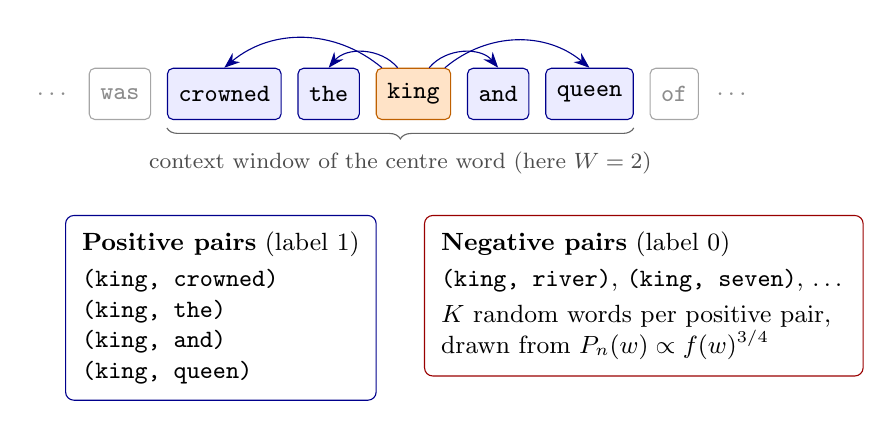
\begin{tikzpicture}[
    tok/.style={draw=black!35, rounded corners=2pt, minimum height=6.5mm, inner xsep=4pt, font=\small\ttfamily, text=black!45},
    ctx/.style={tok, fill=blue!8, draw=blue!55!black, text=black},
    ctr/.style={tok, fill=orange!22, draw=orange!75!black, text=black, font=\small\ttfamily\bfseries},
    pairbox/.style={draw, rounded corners=3pt, align=left, inner sep=6pt, font=\small},
    >={Stealth[length=2mm]}
]
    \node[tok] (t1) {was};
    \node[ctx, right=2mm of t1] (t2) {crowned};
    \node[ctx, right=2mm of t2] (t3) {the};
    \node[ctr, right=2mm of t3] (t4) {king};
    \node[ctx, right=2mm of t4] (t5) {and};
    \node[ctx, right=2mm of t5] (t6) {queen};
    \node[tok, right=2mm of t6] (t7) {of};
    \node[left=1mm of t1, font=\small, text=black!45] {\dots};
    \node[right=1mm of t7, font=\small, text=black!45] {\dots};

    \draw[->, blue!55!black] ([xshift=-2mm]t4.north) to[bend right=50] (t3.north);
    \draw[->, blue!55!black] ([xshift=-4mm]t4.north) to[bend right=40] (t2.north);
    \draw[->, blue!55!black] ([xshift=2mm]t4.north) to[bend left=50] (t5.north);
    \draw[->, blue!55!black] ([xshift=4mm]t4.north) to[bend left=40] (t6.north);

    \draw[decorate, decoration={brace, mirror, amplitude=4pt}, black!60]
        ([yshift=-1mm]t2.south west) -- ([yshift=-1mm]t6.south east)
        node[midway, below=5pt, font=\footnotesize, text=black!70] (win) {context window of the centre word (here $W = 2$)};

    \node[pairbox, draw=blue!55!black, anchor=north east] (pos) at ([xshift=-3mm, yshift=-4mm]win.south)
        {\textbf{Positive pairs} (label 1)\\[2pt]
         \texttt{(king, crowned)}\\ \texttt{(king, the)}\\ \texttt{(king, and)}\\ \texttt{(king, queen)}};
    \node[pairbox, draw=red!60!black, anchor=north west] (neg) at ([xshift=3mm, yshift=-4mm]win.south)
        {\textbf{Negative pairs} (label 0)\\[2pt]
         \texttt{(king, river)}, \texttt{(king, seven)}, \dots\\[2pt]
         $K$ random words per positive pair,\\
         drawn from $P_n(w) \propto f(w)^{3/4}$};
\end{tikzpicture}
}
    \end{center}
    \vspace{1mm}
    \begin{itemize}
        \item Window size drawn at random, $W \sim U\{1, \dots, 5\}$: nearby words count more
        \item About 6 positive pairs per centre word
    \end{itemize}
\end{frame}

% ---------------------------------------------------------------- 5
\begin{frame}{Negative sampling: a binary task instead of a softmax}
    \muted{Mikolov et al. (2013b)}: tell the true pair apart from $K$ random pairs
    \[
        \underbrace{\log \sigma(\mathbf{v}'_o \cdot \mathbf{v}_c)}_{\text{pull the true context closer}}
        \; + \;
        \underbrace{\sum_{k=1}^{K} \log \sigma(-\mathbf{v}'_{n_k} \cdot \mathbf{v}_c)}_{\text{push random words away}},
        \qquad n_k \sim P_n(w) \propto f(w)^{3/4}
    \]
    \begin{itemize}
        \item Cost per pair: $O(K)$ with $K = 5$, instead of $O(V)$
        \item The exponent $3/4$ samples rare words more often than their raw frequency
        \item \textbf{Subsampling}: drop occurrences of very frequent words (\textit{the}, \textit{of}) with probability $1 - \sqrt{t / f(w)}$
    \end{itemize}
\end{frame}

% ---------------------------------------------------------------- 6
\begin{frame}{Implementation}
    \begin{center}
        \resizebox{\textwidth}{!}{% Training and evaluation pipeline with the code location of each stage (shared by report and slides).
% Requires \usetikzlibrary{positioning,arrows.meta}
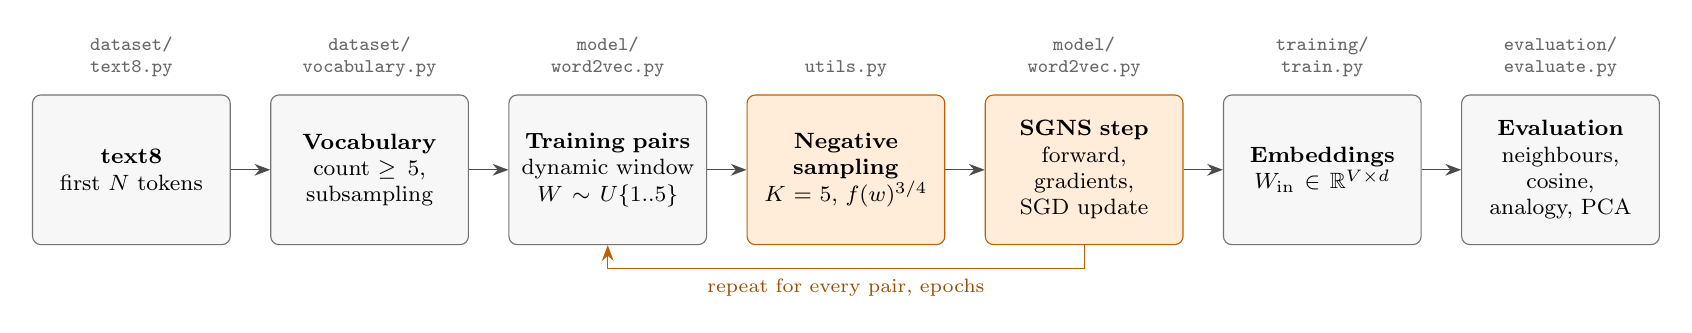
\begin{tikzpicture}[
    stage/.style={draw=black!55, rounded corners=3pt, fill=black!3, align=center, minimum height=19mm,
                  text width=23mm, inner sep=3pt, font=\footnotesize},
    model/.style={stage, fill=orange!15, draw=orange!75!black},
    file/.style={font=\scriptsize\ttfamily, text=black!60, align=center, text width=24mm, anchor=south},
    >={Stealth[length=2mm]}
]
    \node[stage] (s1) {\textbf{text8}\\first $N$ tokens};
    \node[stage, right=5mm of s1] (s2) {\textbf{Vocabulary}\\count $\geq 5$,\\subsampling};
    \node[stage, right=5mm of s2] (s3) {\textbf{Training pairs}\\dynamic window\\$W \sim U\{1..5\}$};
    \node[model, right=5mm of s3] (s4) {\textbf{Negative}\\\textbf{sampling}\\$K = 5$, $f(w)^{3/4}$};
    \node[model, right=5mm of s4] (s5) {\textbf{SGNS step}\\forward, gradients,\\SGD update};
    \node[stage, right=5mm of s5] (s6) {\textbf{Embeddings}\\$W_{\text{in}} \in \mathbb{R}^{V \times d}$};
    \node[stage, right=5mm of s6] (s7) {\textbf{Evaluation}\\neighbours, cosine,\\analogy, PCA};

    \foreach \a/\b in {s1/s2, s2/s3, s3/s4, s4/s5, s5/s6, s6/s7}
        \draw[->, black!70] (\a) -- (\b);
    \draw[->, orange!75!black] (s5.south) -- ++(0,-3mm) -| node[pos=0.25, below, font=\scriptsize, text=orange!60!black] {repeat for every pair, epochs} (s3.south);

    \node[file, above=1mm of s1] {dataset/\\text8.py};
    \node[file, above=1mm of s2] {dataset/\\vocabulary.py};
    \node[file, above=1mm of s3] {model/\\word2vec.py};
    \node[file, above=1mm of s4] {\\utils.py};
    \node[file, above=1mm of s5] {model/\\word2vec.py};
    \node[file, above=1mm of s6] {training/\\train.py};
    \node[file, above=1mm of s7] {evaluation/\\evaluate.py};
\end{tikzpicture}
}
    \end{center}
    \small
    \muted{NumPy SGNS from the open-source repository of Caselli (2026). Our additions:}
    \vspace{1mm}
    \begin{columns}[T]
        \begin{column}{0.32\textwidth}
            \textbf{Reproducible runs}\\
            seed, every hyperparameter on the CLI, \texttt{config.json} per run; fixed the documented command
        \end{column}
        \begin{column}{0.32\textwidth}
            \textbf{4$\times$ faster training}\\
            negatives drawn in batches from the same distribution: 1,023\,s $\to$ 251\,s on 1M tokens, same losses
        \end{column}
        \begin{column}{0.32\textwidth}
            \textbf{Evaluation protocol}\\
            queries fixed in advance, untrained baseline, frequency-matched cosine percentiles
        \end{column}
    \end{columns}
\end{frame}

% ---------------------------------------------------------------- 7
\begin{frame}{Results: training loss and nearest neighbours}
    \begin{columns}[T]
        \begin{column}{0.46\textwidth}
            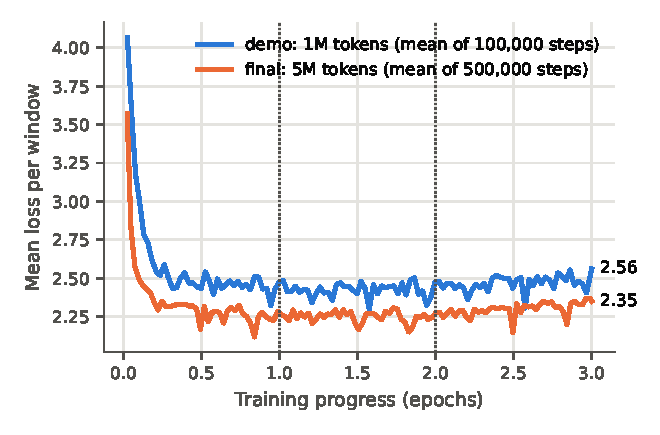
\includegraphics[width=\linewidth]{loss_curves_slides.pdf}
            \small
            \begin{itemize}
                \item Falls early in epoch 1, then flat
                \item Epoch means \FinalLossEpochOne{} $\to$ \FinalLossEpochTwo{} $\to$ \FinalLossEpochThree\\
                      $\Rightarrow$ loss is \hl{not} a quality measure
            \end{itemize}
        \end{column}
        \begin{column}{0.52\textwidth}
            \resizebox{\linewidth}{!}{% Generated by experiments/make_report_assets.py; do not edit by hand.
\begin{tabular}{ll}
\toprule
Query & Nearest neighbours (top 4) \\
\midrule
\textit{king} & alexius, grandson, throne, vii \\
\textit{computer} & computers, computing, interface, hardware \\
\textit{city} & town, edmonton, bronx, bremerhaven \\
\textit{france} & italy, spain, netherlands, switzerland \\
\textit{january} & february, december, october, june \\
\textit{three} & seven, four, six, two \\
\textit{war} & peloponnesian, ww, wwii, outbreak \\
\textit{music} & jazz, musical, dance, pop \\
\bottomrule
\end{tabular}
}
            \vspace{2mm}

            \small Final run (\FinalTokensShort{} tokens); queries fixed in advance.\\
            \muted{Untrained model: \textit{king} $\to$ \textit{marpat, verbally, brando}}
        \end{column}
    \end{columns}
\end{frame}

% ---------------------------------------------------------------- 8
\begin{frame}[fragile]{Live demo: similarity, analogies, visualisation}
    \begin{columns}[T]
        \begin{column}{0.5\textwidth}
            \texttt{\$ python demo/demo.py}
            \vspace{2mm}
            \footnotesize
\begin{verbatim}
> king queen
  0.699: more similar than 99.7%
         of random frequent-word pairs
> king software
  0.123: more similar than 5.0%

> bigger - big + small
  smaller  parking  forested
> king - man + woman
  daughter  caligula  amalric
\end{verbatim}
            \small
            Analogies: \hl{\FinalHitOne/\FinalAnswerable} exact, \FinalHitFive/\FinalAnswerable{} in top 5\\
            \muted{(1M tokens: \DemoHitOne{} and \DemoHitFive; untrained: 0)}
        \end{column}
        \begin{column}{0.48\textwidth}
            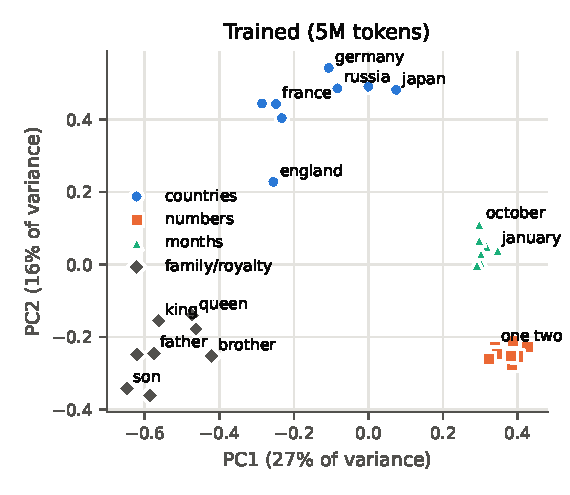
\includegraphics[width=\linewidth]{pca_final_trained.pdf}
        \end{column}
    \end{columns}
\end{frame}

% ---------------------------------------------------------------- 9
\begin{frame}{Conclusion}
    \small
    \begin{tabular}{@{}l>{\raggedright\arraybackslash}p{0.72\textwidth}@{}}
        \toprule
        \textbf{Q1} Loss & drops early, then flat; says little about embedding quality \\
        \textbf{Q2} Neighbours & \hl{yes}: months, numbers, countries, genres cluster \\
        \textbf{Q3} Similarity & \hl{yes}, against the right baseline: related pairs $\geq$ p\FinalRelatedPctMin, controls $\leq$ p\FinalControlPctMax \\
        \textbf{Q4} Analogies & \hl{partly}: \FinalHitOne/\FinalAnswerable{} exact; \textit{king} $-$ \textit{man} $+$ \textit{woman} $\not\to$ \textit{queen} \\
        \textbf{Q5} Space & \hl{yes}: four word groups form separate clusters in 2D \\
        \bottomrule
    \end{tabular}
    \vspace{5mm}
    \begin{columns}[T]
        \begin{column}{0.48\textwidth}
            \textbf{Limitations}
            \begin{itemize}
                \item 5M tokens, a prefix of Wikipedia
                \item rare words barely trained
                \item one vector per word (\textit{bank})
                \item small fixed evaluation, one seed
            \end{itemize}
        \end{column}
        \begin{column}{0.48\textwidth}
            \textbf{Applications}
            \begin{itemize}
                \item input features for text classifiers
                \item similarity search, query expansion
                \item exploring how a corpus uses words
            \end{itemize}
        \end{column}
    \end{columns}
\end{frame}

% ================================================================ backup
\begin{frame}[plain]
    \vfill
    \centering
    {\usebeamercolor[fg]{title}\LARGE\bfseries Backup slides\par}
    \vfill
\end{frame}

\begin{frame}{Backup: runs and hyperparameters}
    \begin{columns}[T]
        \begin{column}{0.42\textwidth}
            \resizebox{\linewidth}{!}{% Generated by experiments/make_report_assets.py; do not edit by hand.
\begin{tabular}{lrr}
\toprule
 & Demo & Final \\
\midrule
Tokens of text8 & 1,000,000 & 5,000,000 \\
Vocabulary size & 13,966 & 36,280 \\
Tokens after subsampling & 635,140 & 3,372,979 \\
Training steps (pairs) & 11,425,544 & 60,708,682 \\
Training time & 4.2 min & 24.7 min \\
Throughput (steps/s) & 45,500 & 40,900 \\
\midrule
Mean loss, epoch 1 & 2.591 & 2.347 \\
Mean loss, epoch 2 & 2.424 & 2.250 \\
Mean loss, epoch 3 & 2.468 & 2.299 \\
\midrule
Random-pair cosine (top 2,000) & 0.61 $\pm$ 0.19 & 0.32 $\pm$ 0.12 \\
Analogies: hit@1 / hit@5 & 0 / 2 of 8 & 4 / 6 of 8 \\
\bottomrule
\end{tabular}
}
        \end{column}
        \begin{column}{0.56\textwidth}
            \resizebox{\linewidth}{!}{% Generated by experiments/make_report_assets.py; do not edit by hand.
\begin{tabular}{lll}
\toprule
Hyperparameter & Value & CLI option \\
\midrule
Tokens of text8 used & 1,000,000 (demo) / 5,000,000 (final) & \texttt{--max-tokens} \\
Minimum word count & 5 & \texttt{--min-count} \\
Subsampling threshold $t$ & 0.001 & \texttt{--subsample-t} \\
Embedding dimension $d$ & 100 & \texttt{--embed-dim} \\
Epochs & 3 & \texttt{--epochs} \\
Maximum window size & 5 & \texttt{--max-window} \\
Negative samples $K$ & 5 & \texttt{--n-negatives} \\
Noise distribution exponent & 0.75 & fixed \\
Initial / minimum learning rate & 0.025 / 0.0001 & \texttt{--start-lr}, \texttt{--lr-min} \\
Loss report interval (steps) & 100,000 / 500,000 & \texttt{--report-every} \\
Random seed & 42 & \texttt{--seed} \\
\bottomrule
\end{tabular}
}
        \end{column}
    \end{columns}
    \vspace{3mm}
    \small Apple M5, one core, Python \FinalPython, NumPy \FinalNumpy. Same arguments $\Rightarrow$ identical embeddings.
\end{frame}

\begin{frame}{Backup: cosine similarity needs a baseline}
    \begin{columns}[T]
        \begin{column}{0.55\textwidth}
            \resizebox{\linewidth}{!}{% Generated by experiments/make_report_assets.py; do not edit by hand.
\begin{tabular}{lrrr}
\toprule
Pair & Demo (1M) & Final (5M) & Untrained \\
\midrule
\textit{king} -- \textit{queen} & 0.91 (p98) & 0.70 (p100) & 0.10 (p82) \\
\textit{man} -- \textit{woman} & 0.89 (p97) & 0.77 (p100) & $-$0.06 (p30) \\
\textit{computer} -- \textit{software} & 0.80 (p84) & 0.75 (p100) & 0.17 (p96) \\
\textit{city} -- \textit{country} & 0.78 (p81) & 0.45 (p85) & $-$0.14 (p9) \\
\textit{france} -- \textit{germany} & 0.86 (p93) & 0.76 (p100) & 0.05 (p68) \\
\textit{january} -- \textit{february} & 0.95 (p100) & 0.91 (p100) & $-$0.03 (p39) \\
\midrule
\textit{king} -- \textit{software} & 0.14 (p1) & 0.12 (p5) & 0.00 (p49) \\
\textit{computer} -- \textit{january} & 0.42 (p17) & 0.18 (p12) & 0.04 (p67) \\
\textit{music} -- \textit{france} & 0.42 (p18) & 0.25 (p32) & 0.05 (p69) \\
\bottomrule
\end{tabular}
}
        \end{column}
        \begin{column}{0.42\textwidth}
            \small
            \begin{itemize}
                \item pN: more similar than N\% of random pairs among the \BaselineWords{} most frequent words
                \item Random frequent pairs average \DemoBaselineMean{} (1M) and \FinalBaselineMean{} (5M)
                \item Over the whole vocabulary: \FinalBaselineAllMean{}, because rare words stay near a shared direction
                \item Baseline changed to frequent words \hl{after} the first demo evaluation; queries unchanged
            \end{itemize}
        \end{column}
    \end{columns}
\end{frame}

\begin{frame}{Backup: all fixed analogies}
    \centering
    \resizebox{0.95\textwidth}{!}{% Generated by experiments/make_report_assets.py; do not edit by hand.
\begin{tabular}{lllrrr}
\toprule
 & & & \multicolumn{3}{c}{Rank of expected} \\
\cmidrule(l){4-6}
Analogy & Expected & Final: top 3 & Final & Demo & Untrained \\
\midrule
\textit{man} : \textit{king} :: \textit{woman} : ? & \textit{queen} & daughter, caligula, amalric & $>$10 & $>$10 & $>$10 \\
\textit{france} : \textit{paris} :: \textit{italy} : ? & \textit{rome} & interred, venice, geneva & $>$10 & $>$10 & $>$10 \\
\textit{france} : \textit{paris} :: \textit{germany} : ? & \textit{berlin} & berlin, munich, exposition & 1 & $>$10 & $>$10 \\
\textit{man} : \textit{woman} :: \textit{boy} : ? & \textit{girl} & baby, girl, marple & 2 & $>$10 & $>$10 \\
\textit{brother} : \textit{sister} :: \textit{father} : ? & \textit{mother} & mother, grandfather, parents & 1 & $>$10 & $>$10 \\
\textit{good} : \textit{better} :: \textit{bad} : ? & \textit{worse} & fare, worse, cheaper & 2 & $>$10 & $>$10 \\
\textit{big} : \textit{bigger} :: \textit{small} : ? & \textit{smaller} & smaller, parking, forested & 1 & 3 & $>$10 \\
\textit{england} : \textit{english} :: \textit{france} : ? & \textit{french} & french, spanish, portuguese & 1 & 5 & $>$10 \\
\bottomrule
\end{tabular}
}
    \vspace{3mm}

    \small Expected answer $\approx \mathbf{v}_b - \mathbf{v}_a + \mathbf{v}_c$, excluding $a$, $b$, $c$; rank among the ten best candidates.
\end{frame}

\begin{frame}{Backup: embedding space before and after training}
    \centering
    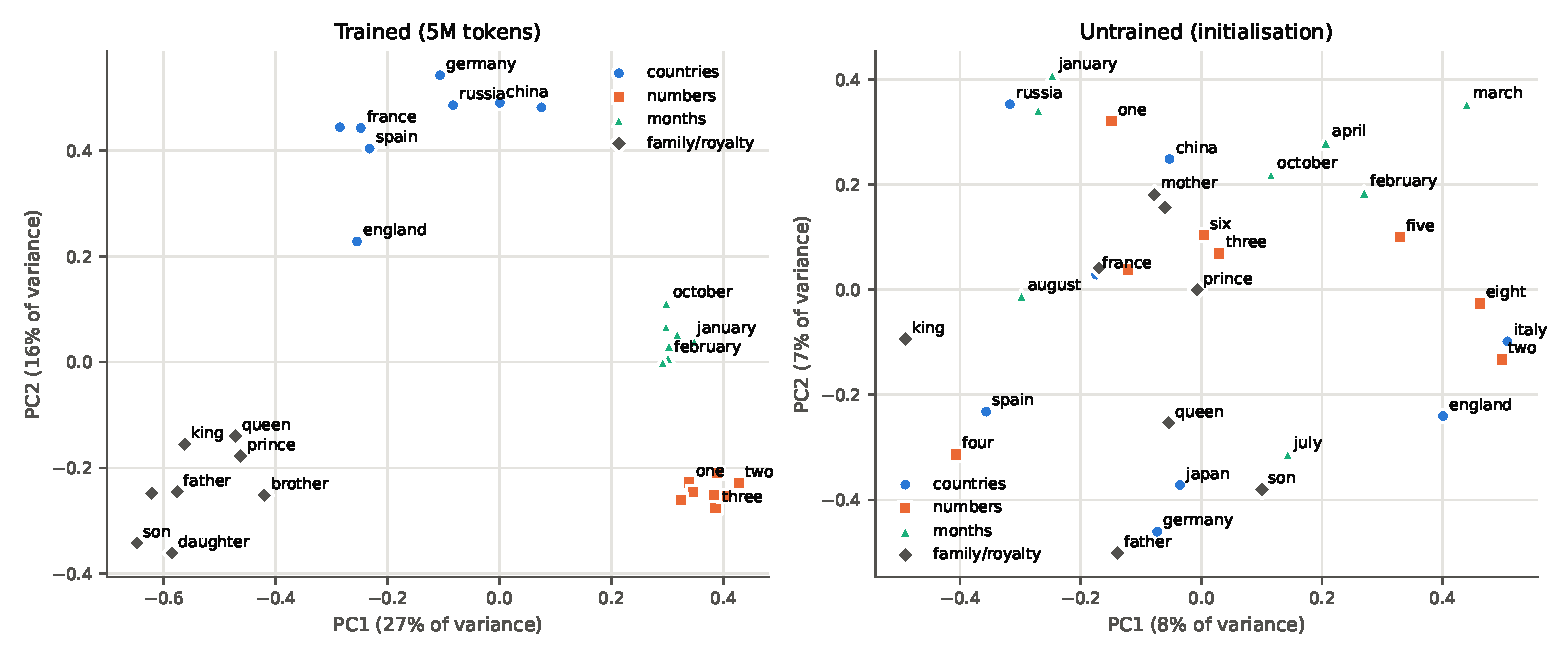
\includegraphics[width=0.95\textwidth]{pca_final.pdf}
\end{frame}

\begin{frame}{References}
    \footnotesize
    \begin{itemize}
        \item N.~Caselli (2026). \textit{word2vec-from-scratch}. GitHub repository, \texttt{github.com/NiccoloCase/word2vec-from-scratch}.
        \item J.~R.~Firth (1957). A synopsis of linguistic theory, 1930--1955. \textit{Studies in Linguistic Analysis}.
        \item Y.~Goldberg, O.~Levy (2014). word2vec explained. arXiv:1402.3722.
        \item Z.~S.~Harris (1954). Distributional structure. \textit{Word} 10(2--3).
        \item M.~Mahoney. About the test data (text8). \texttt{mattmahoney.net/dc/textdata.html}.
        \item T.~Mikolov, K.~Chen, G.~Corrado, J.~Dean (2013a). Efficient estimation of word representations in vector space. arXiv:1301.3781.
        \item T.~Mikolov, I.~Sutskever, K.~Chen, G.~Corrado, J.~Dean (2013b). Distributed representations of words and phrases and their compositionality. \textit{NeurIPS}.
        \item T.~Mikolov, W.~Yih, G.~Zweig (2013c). Linguistic regularities in continuous space word representations. \textit{NAACL-HLT}.
        \item J.~Mu, P.~Viswanath (2018). All-but-the-top: simple and effective postprocessing for word representations. \textit{ICLR}.
    \end{itemize}
\end{frame}

\end{document}
